\sect{Casos de uso}{casos_de_uso}

En un proyecto software, los casos de uso son una técnica para la captura de requisitos de un sistema~\cite{use_cases}.
Un caso de uso describe una unidad discreta de trabajo que puede ser realizada por el sistema, formada por un conjunto
de acciones que el sistema realiza.\ El siguiente diagrama representa los casos de uso básicos detectados para
la aplicación:

\begin{figure}[H]
	\centering
	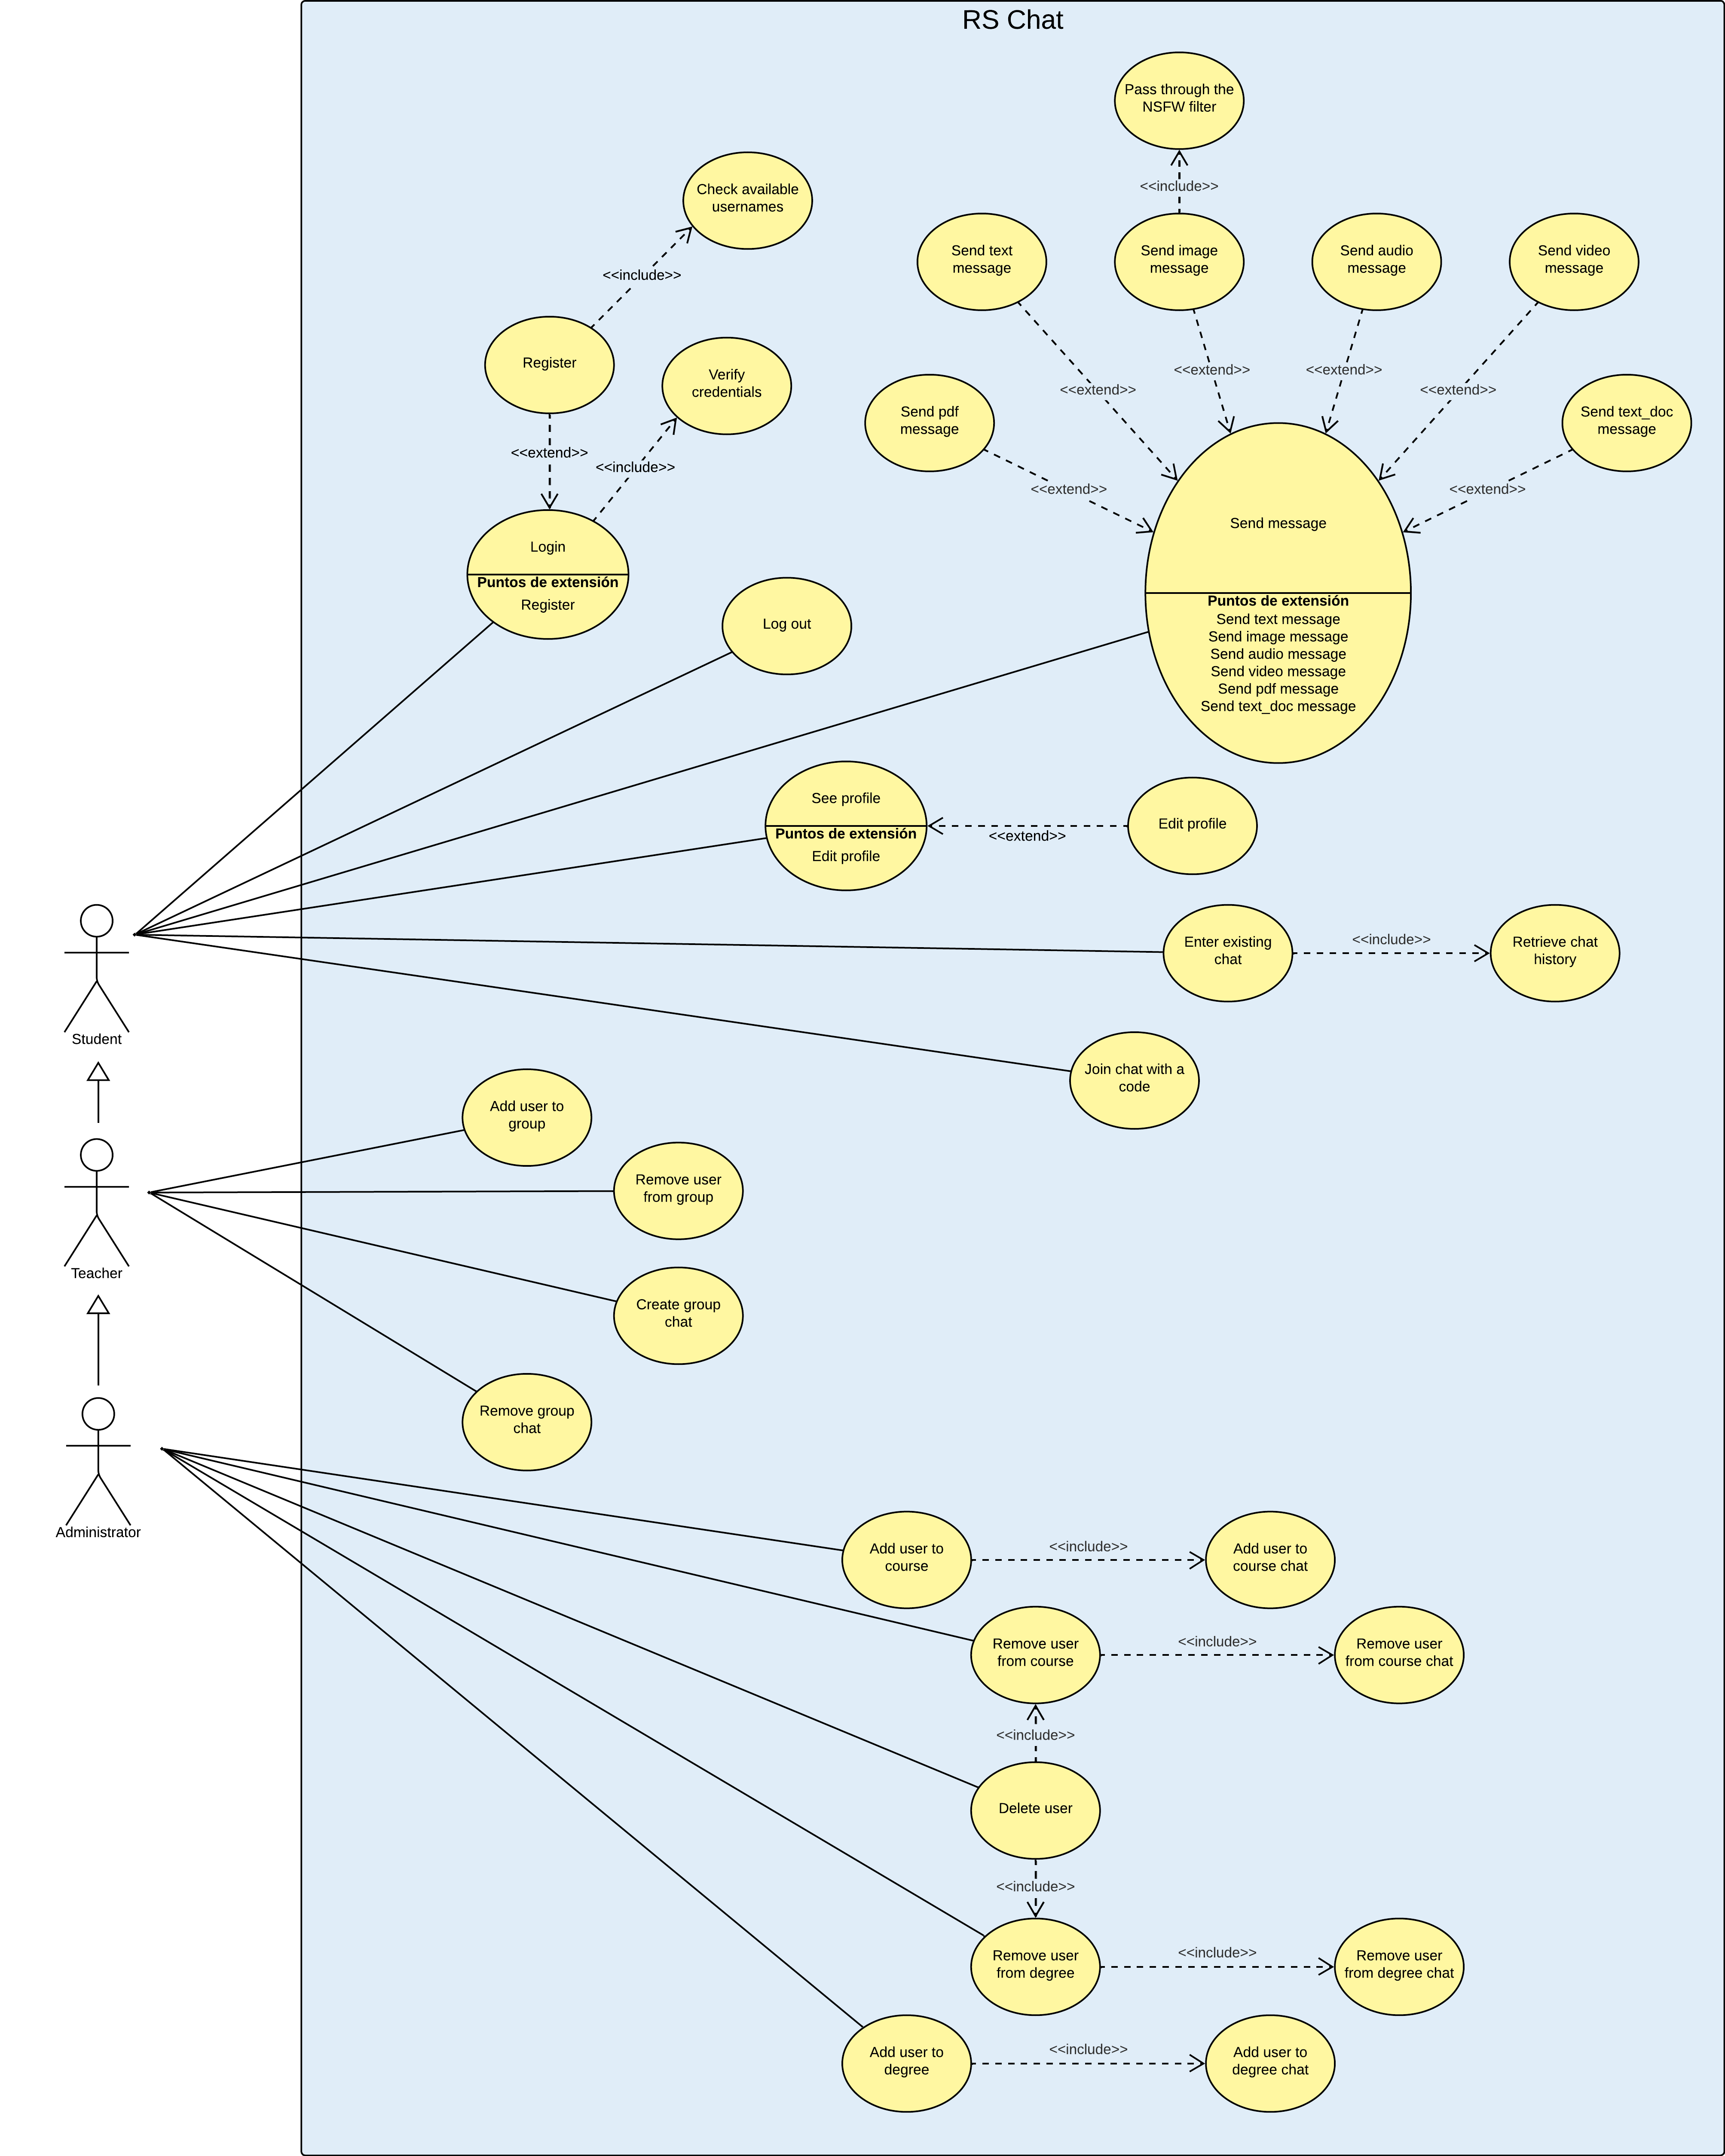
\includegraphics[width=0.8\textwidth]{res/images/RSChat-Diagrams-Usecases}
	\caption{Diagrama de casos de uso.}
	\label{fig:casosDeUso}
\end{figure}
